Figure \ref{fig:zonal_LEV_radius_Re200k} shows the radius of the LEV for different meshes at multiple phases.
Recall that LEV radius is considered to be
the radial distance from center of LEV core where maximum tangential velocity is achieved, and this tangential velocity is computed along multiple radial lines, and the peak tangential
velocity is obtained from this averaged tangential velocity along multiple radial lines.

M0\_nz50 mesh shows the largest radius among all the meshes, and fails to capture the trend that the other finer meshes show.
Mza1\_nz50 mesh follows a similar trend as Mza2\_nz50 mesh.
Mza2\_nz50 shows the lowest radius among all the meshes, which is expected as mesh resolution is highest in this mesh, and as a result, a less diffused LEV is resolved.


\begin{figure}[H]
	\centering
	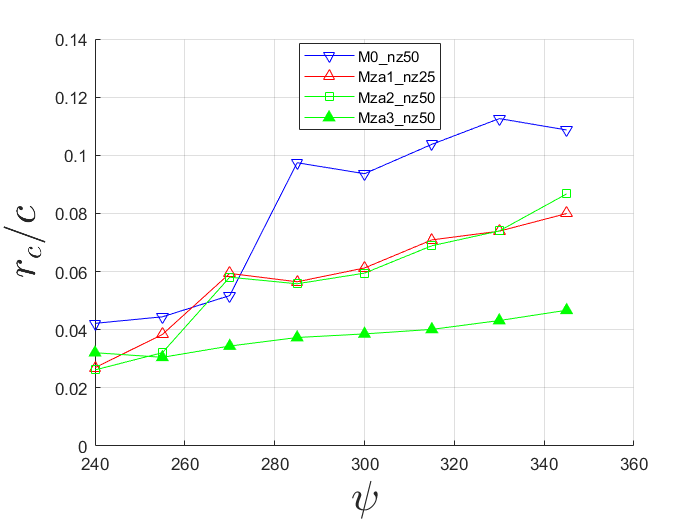
\includegraphics[width=0.7\textwidth]{figures/zonal_adapt_results/LEV_Re200k/LEV_radius_vp}
	\caption{ LEV radius for different meshes}
	\label{fig:zonal_LEV_radius_Re200k}
\end{figure}

Figure \ref{fig:zonal_LEV_location_Re200k} shows the location of the center of the LEV core for different phases after it is ejected from the airfoil surface.
Note that the LEV is ejected closer to the trailing edge as compared to the lower Reynolds number of $Re=40,000$, for the same advance ratio.
M0\_nz50 mesh shows differences for LEV path from Mza1\_nz50 and Mza2\_nz50 meshes. LEV shows a similar path for Mza1\_nz50 and Mza2\_nz50 meshes.

\begin{figure}[H]
	\centering
	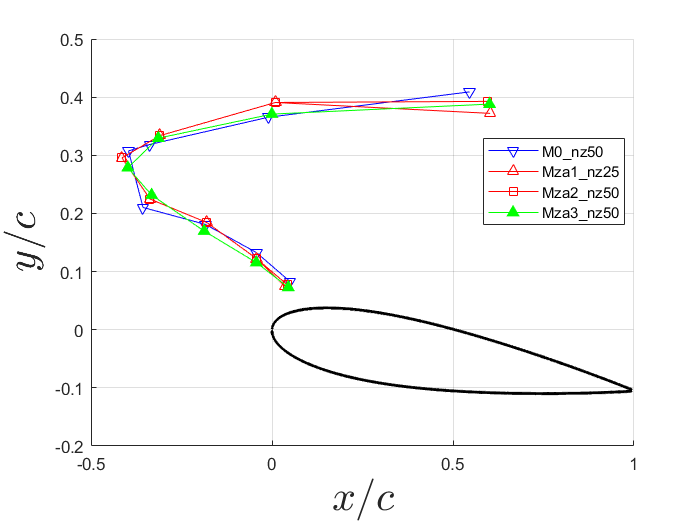
\includegraphics[width=0.75\textwidth]{figures/zonal_adapt_results/LEV_Re200k/LEV_location_Re200k}
	\caption{ LEV location for different meshes}
	\label{fig:zonal_LEV_location_Re200k}
\end{figure}
